
%%%%%%%%%%%%%%%%%%%%%%%%%%%%%%%%%%%%%%%%%%%%%%%%%%%%%%%%%%%%%%%%%%%%%%%%%%%%%%%%
%%%%%%%%%%%%%%%%%%%%%%%%%%%%%%%%%%%%%%%%%%%%%%%%%%%%%%%%%%%%%%%%%%%%%%%%%%%%%%%%
% INTRODUCTION %
%%%%%%%%%%%%%%%%%%%%%%%%%%%%%%%%%%%%%%%%%%%%%%%%%%%%%%%%%%%%%%%%%%%%%%%%%%%%%%%%

\cleardoublepage
\chapter{Introduction}
\label{sec:intro}
\pagenumbering{arabic} % para empezar la numeración de página con números

Computational thinking (CT) is a knowledge field of great relevance and interest nowadays. During the last decade, CT has become more significant in sectors as important as education. However, to get an exact definition about CT is an actual challenge. In the year 2006, Wing defined CT as a process of formulation and resolution of problems which employs the fundamental concepts of computing~\cite{wing:_ct}. Although its skills can be developed in different ways, one of the most common tools to learn it, train it and develop it, is through programming. In this chapter, we describe the importance of an appropriate development of CT skills and how Scratch can be a fundamental tool for it. 


\section{General context}
\label{sec:context}

The new technologies represent a fundamental role in the daily life of children and teenagers. In addition, the fact that technologies are still growing, developing and becoming more important and necessary, is a certainty. In this new era, programming is an essential knowledge. 

Learning how to program since childhood is like learning a new language, the earlier children start, the easier it will be for them to acquire its skills and abilities.

Therefore, when we talk about programming, the intention is not that children learn advanced concepts since childhood. The main purpose in these early ages is that they participate in the digital world in a secure, responsible and conscious way. In this way, new generations will be able to understand the new technologies and use them to solve problems in their quotidian life. The main objective of teaching programming in the classrooms is that students obtain the necessary tools to manage themselves in a technological world~\cite{mangifesta:_importancia}. 

The inclusion of programming in the educational field allows the development of computational thinking. CT is composed of different skills which are very necessary for children, such as abstraction, logic or problem decomposition. In this way, CT should be considered an ability as important as the reading, writing or mathematics in the schools ~\cite{calao:_design}.

However, from software engineering, we know that problems solved through programming may have not been solved in the most appropriate way. These symptoms or bad practice are known as ``bad smells''. In other words, the program may run and may even solve the problem, but it contains elements that make it difficult to understand, to modify and to reuse~\cite{zhang:_badsmells}. Martin defines code smells as follows~\cite{martin:_clean}: ``Code smells are usually not bugs; they are not technically incorrect and do not prevent the program from functioning. Instead, they indicate weaknesses in design that may slow down development or increase the risk of bugs or failures in the future''. Despite the negative effect they produce, bad smells have been little investigated and analyzed in CT research. As Hermans and Aivaloglou have found in an experiment with Scratch learners ~\cite{felienne:_hamper}, we argue that bad smells hinder the proper development of CT skills in learners. Their identification should be a first step towards guiding learners towards good practices that offer them the possibility to develop themselves to their full potential.

Years ago, learning to program was a complicated task. The information to start this process was scarcer and the programming languages less intuitive. Programming based on best practice was even more complicated. Nowadays, there are numerous tools and languages to begin in the world of programming and computational thinking. In the following section, we describe Scratch, a visual language of programming designed for children and beginners, which is already used by millions of students worldwide.


\section{Scratch}
\label{sec:scratch}

Scratch~\footnote{https://scratch.mit.edu/} is a visual programming language oriented to education. It has been designed by the MIT to facilitate the learning in an intuitive way, through the use of blocks. The greatest virtue of Scratch is to allow to create stories, games or animations without previous programming knowledge.

Instead of using the conventional code, the huge revolution of Scratch is the use of different pieces or blocks. The blocks are grouped by clearly identified categories, with different colors. The main functionality is based on the creation of structures with these blocks and the generation of necessary instructions so that the program works. In this way, learning to program is easier and more entertaining.

In addition, the last January of 2019 was launched Scratch 3.0, a new version which includes new categories and functionalities. With this update, Scratch has improved its variety of blocks. Its new web interface is shown in the figure ~\ref{fig:scratch}.


\begin{figure}[h]
  \centering
  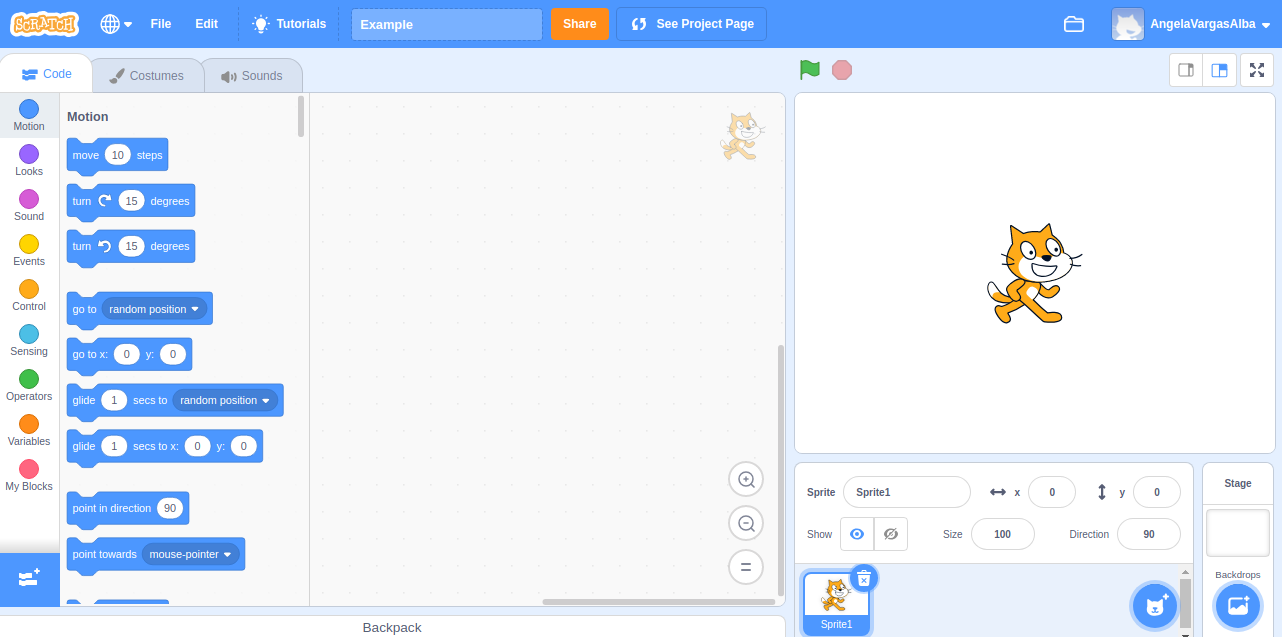
\includegraphics[width=9cm, keepaspectratio]{img/scratch.png}
  \caption{Web interface of Scratch 3.0.}
  \label{fig:scratch}
\end{figure}

On the other hand, Scratch is a world community. In this collaborative space, the ``scratchers'' can interact and share their projects, to analyze them or to remix them. In addition, they can explain their doubts in a forum or comment other projects. In this way, beginner programmers can learn in a dynamic way, with the help of other programmers. In the figure ~\ref{fig:statistics_scratch} we can observe the statistics on October 2019. Scratch is an amazing community that also continues to grow. 

\begin{figure}[h]
  \centering
  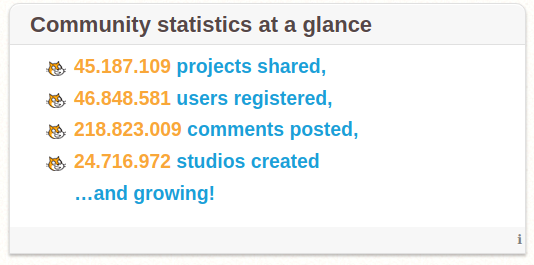
\includegraphics[width=9cm, keepaspectratio]{img/statistics_scratch.png}
  \caption{Statistics of the Scratch community.}
  \label{fig:statistics_scratch}
\end{figure}



\section{Frame of reference}
\label{sec:reference}

With the growth of Scratch and its impact in the educational field, my tutor of this project - Dr. Gregorio Robles - together with the Dr. Jesús Moreno observed the need of a tool to evaluate the Scratch projects. In this way, Dr. Scratch~\footnote{http://www.drscratch.org/} was created in 2014.

Dr. Scratch is a web application which allows both teachers and students to automatize the analysis of Scratch projects in order to verify if the projects have been programmed correctly, to verify the bad practice in the code, to learn from their errors, to receive feedback or to improve the code. Its main interface web is shown in the figure~\ref{fig:dr_scratch}.

\begin{figure}[h]
  \centering
  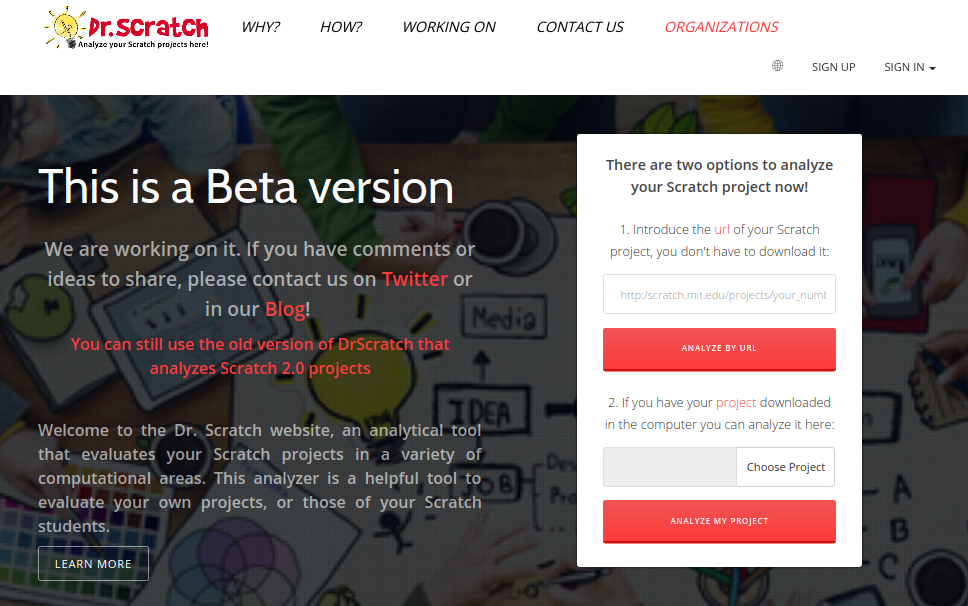
\includegraphics[width=9cm, keepaspectratio]{img/dr_scratch.png}
  \caption{Interface web of Dr.Scratch.}
  \label{fig:dr_scratch}
\end{figure}

In order to analyze a project, Dr. Scratch utilizes the files generated with Scratch. These files have a compressed format and contain a JSON file with the relevant information about the blocks utilized. In the previous version, the extension of these files was \textit{.sb2}. When we initiated this project, we knew that this format would be changed by the extension \textit{.sb3} in the new version Scratch 3.0. In addition, the content of these JSON files would change significantly. Therefore, one of the main challenges of this project was the adaptation of Dr.Scratch to the new version Scratch 3.0 which would be launched. 

For the analysis of the projects, Dr. Scratch used \textit{Hairball}~\footnote{https://github.com/jemole/hairball}, a plugin framework. The essential objective of the update was to simplify the tool, removing Hairball and integrating their functionality in the code. Therefore, the starting point was to adapt Dr.Scratch to the new version Scratch 3.0, getting the same functionalities, but with the new files \textit{.sb3} and without the Hairball module.

Once the projects are analyzed, Dr. Scratch shows different dashboards with the results, which can be observed in the figure ~\ref{fig:dashboards}.

\begin{figure}[h]
  \centering
  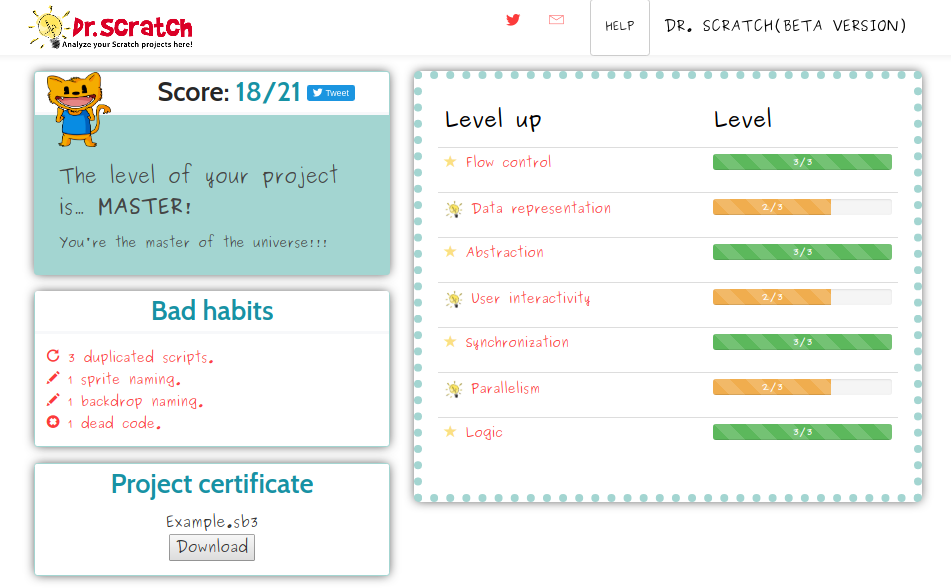
\includegraphics[width=9cm, keepaspectratio]{img/dashboards.png}
  \caption{Dashboards of Dr. Scratch with the result of the analysis.}
  \label{fig:dashboards}
\end{figure}

In order to measure the development grade of CT demonstrated in programming, Dr.Scratch gives a numeric punctuation based on the level reached in seven categories of CT: abstraction, logical thinking, synchronization, parallelism, flow control, user interactivity and data representation ~\cite{jesus:_drscratch}. Each of these capacities receives a punctuation from 0 to 3 points, depending on the Scratch blocks used. In this way, the final score varies between 0 to 21 points, with three different levels of programmers: basic, developing or proficiency.   

In addition, Dr.Scratch analyzes the bad smells that may exist in the code. That is, code that has never been executed (dead code), code that is copied and pasted in the scripts of different characters (repeated code) or the lack of significant naming (default naming). In the previous version, this dashboard was shown in a small space. Another main challenge of this project was to change the importance that bad smells have in Dr. Scratch. To carry out this process, it was necessary a preliminary analysis about the behaviour of bad smells in Scratch projects.

With this analysis, we could verify that bad smells are present in the majority of the Scratch projects and that they have a negative impact in the development of CT skills. From this point, the objective was to raise awareness of their importance. After a deeper and more exhaustive analysis of bad smells, we considered that it was necessary a new specific model for them in Dr. Scratch. The development of the bad smells mode can be observed in the figure ~\ref{fig:bad_smells}.

\begin{figure}[h]
  \centering
  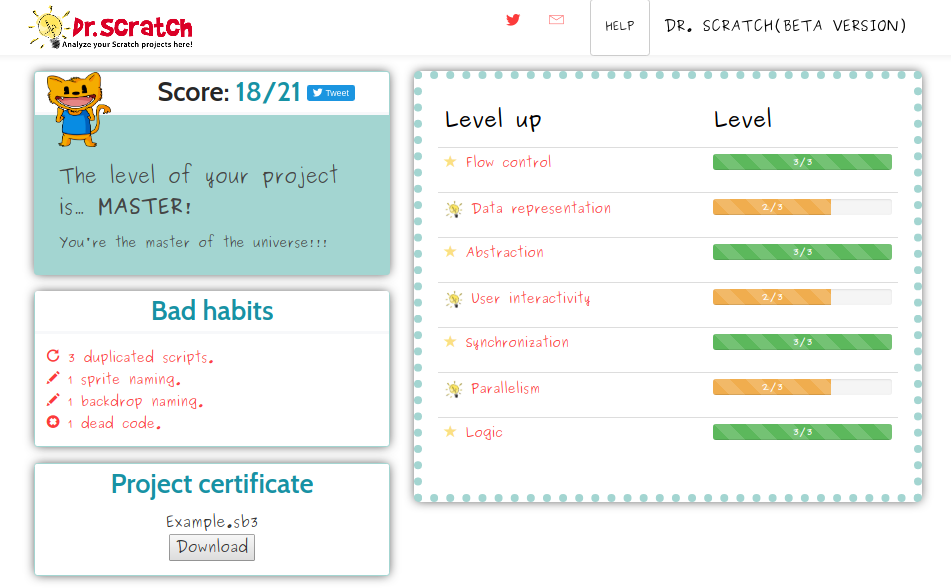
\includegraphics[width=9cm, keepaspectratio]{img/dashboards.png}
  \caption{New model for bad smells in Dr. Scratch [future image].}
  \label{fig:bad_smells}
\end{figure}

The last phase of the project was to prove the effectiveness of this new model in the negative impact of bad smells. After its development, we did an experiment to verify if this new dashboard decreased the number of bad smells present in Scratch projects.


\section{Motivation}
\label{sec:motivation}

Nowadays, there is a lack of resources to introduce CT, in particular programming, in the educational field. In many countries is already being implanted this area as a mandatory subject in schools. However, a lot of teachers do not have enough formation to teach in the most appropriate way this academic world. 

To teach children some good methods of programming and how to avoid bad practice, is one of the most difficult tasks to begin the development of CT. Nowadays, in an era in which programming is at its peak and there is a need to introduce it since childhood, it is very important to do in a responsible and appropriate way since the beginning. 

For this reason, the main motivation of this work has been to analyze in detail the behaviour of bad smells and its evolution. A suitable study about bad smells can help to raise awareness about its presence both in students and teachers, and fostering a more appropriate learning guide.


\section{Structure of the memory}
\label{sec:structure}

Introduce the structure of the memory:

\begin{itemize}
  \item En el primer capítulo se hace una intro al proyecto.
  
  \item En el capítulo~\ref{chap:objectives} se muestran los objetivos del proyecto.
  
  \item A continuación se presenta el estado del arte en el capítulo~\ref{chap:state}.
  
\end{itemize}

